%!TEX root = ../AST208-notes.tex

The levels of the hydrogen atom are shown in Fig.~\ref{f.H-spectrum}.

\begin{figure}[htbp]
\includegraphics[width=\linewidth]{H-spectrum}
\caption{Spectral lines of neutron hydrogen. The first 50 lines for the Lyman ($m\to1$), Balmer ($m\to2$), and Paschen ($m\to3$; note the $4\to2$ transition is outside the plot range) are shown.
\label{f.H-spectrum}}
\end{figure}

\section{Diffraction Gratings}

Figure~\ref{f.slit-and-grating} shows how a spectrum is taken.  A slit is overlaid over the diffraction grating. The dispersed light makes a two dimensional image, with position along the slit along one axis, and wavelength along the other axis.

\begin{figure}[htbp]
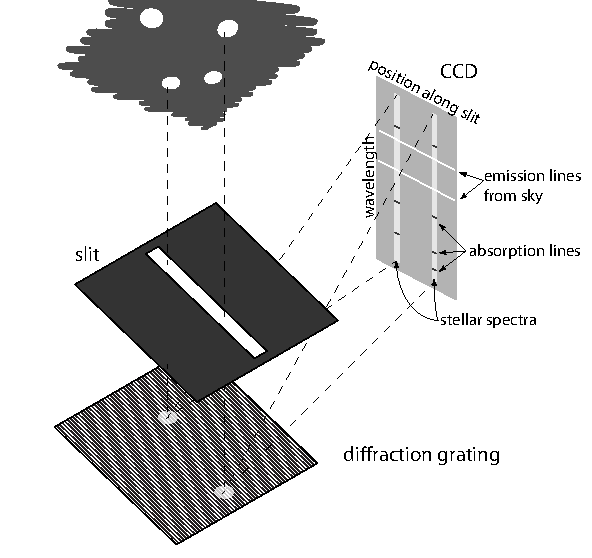
\includegraphics[width=\linewidth]{slit-and-grating}
\caption{Setup for taking a spectrum.
\label{f.slit-and-grating}}
\end{figure} 
